\chapter{Lector/Escritor RFID}\label{anx_antena}

\section{Reglas y Parámetros de Diseño de una Antena RF}

Pasos para el diseño de la antena RF:

\begin{itemize}
\item[A)] Diseñar el inductor, medir su inductancia L y resistencia R (o factor de calidad Q).
\item[B)] Calcular los capacitores para el circuito resonante, que forman junto con el inductor.
\item[C)] Sintonizar el circuito resonante junto con el filtro pasa bajo a la impedancia requerida.
\item[D)] Conectar el circuito resonante a la salida del integrado(TX1 y TX2), verificar la corriente ITVDD y si es necesario sintonizar los componentes para un desempeño óptimo.
\item[E)] Verificar y ajustar el factor de calidad Q.
\item[F)] Verificar y ajustar el circuito receptor.
\end{itemize}

\newpage
\subsection{Diseño del inductor}

Se recomienda usar antenas cuyo inductor tenga forma circular o cuadrado. El valor exacto del inductor es difícil de calcular pero puede ser aproximado por la siguiente ecuación:

\centerline{$ L_{1}[nH]=2 \cdot l_{1} \cdot (ln(\frac{l_{1}}{D_{1}})-K) \cdot N^{1,8}_1$}

\leftline{donde:}
	
\leftline{$l_{1}$ ............... Longitud de una vuelta del conductor (en cm).}

\leftline{$D_{1}$ ............. Diámetro del conductor o ancho del conductor del PCB.}

\leftline{$K$ .............. Factor de forma ($K = 1,07$ antena circular y $K = 1,47$ antena cuadrada).}

\leftline{$N_{1}$ ............. Número de vueltas.}

La antena debe ser simétrica, donde el punto central puede estar conectado a GND. Si esto es así, se sugiere mantener este punto lo más cercano posible al conector de la antena.
El radio de la antena deberá ser $r > 5cm$ para una sola vuelta de cada uno de los inductores simétricos $L_{a}$ y $L_{b}$, o $r < 5cm$ para dos vueltas.
El blindaje de campo eléctrico debe ser conectado a GND.

Los valores de inductancia y resistencia del inductor (fabricado sobre un PCB), si se siguen las reglas de diseño, se encuentran entre: 

$ L = 300nH {...} 2\mu H $

$ R_{coil} =0,5\Omega {...} 5\Omega $


\bigskip
\begin{itshape}
\leftline{Resistor externo}
\end{itshape}


En serie con el inductor se agrega un resistor externo. El valor del mismo se encuentra mediante las ecuaciones:

\centerline{$ Q = \frac{w L}{R_{coil}} \rightarrow R_{coil} = \frac{w L}{Q}$}

\centerline{$ R = 2 \cdot R_{s} + R_{coil} = R_{Sa} + R_{Sb} + R_{coil} $}

donde $R$ es la resistencia total, $R_{Sa}$ y $R_{Sb}$ son cada uno de los resistores externos simétricos.

Definiendo $Q$ entre 20 y 30, se pueden hallar los resistores externos:

$R_{Sa} = R_{Sb} = \frac{1}{2} \cdot (R - R_{coil}) = \frac{wL}{2Q} - \frac{R_{coil}}{2}$ con $w = 2 \pi \cdot 13,56 MHz$


Dejando de lado la influencia de todos los otros componentes en el factor $Q$, este cálculo sólo da una estimación del valor de $R_{S}$, pero esta estimación es necesaria para el cálculo de los capacitores del circuito de resonancia. 

\bigskip
\bigskip
	En muchas aplicaciones prácticas es posible observar que se prescinde del valor de 	resistencia externa $R_{S}$, teniendo en cuenta sólo el valor de resistencia del inductor $R_{coil}$.	

\subsection{Capacitores del circuito resonante}\label{capresonan}
Gracias a la simertría del circuito es posible simplificar los calculos operando sólo con la mitad del circuito, por tanto los valores del inductor $L$, la resistencia $R$ (incluyendo el resistor externo) y el valor de impedancia requerida de la antena $Z_{ant}$, empleados en los siguientes cálculos son la mitad del valor correspondiente a la totalidad del circuito. 
Aplicando entonces la suma de impedancias a la mitad del cirucito y sabiendo que el resultado tiene que ser real e igual a $Z_{ant}$, es posible hallar los valores del capacitor paralelo $C_{2}$ y el capacitor serie $C_{1}$ mediante las siguientes igualdades:

$C_{2a} = C_{2b} = \frac{L}{\omega^{2}L^{2} + R^{2}} - \frac{R}{( \omega^{2}L^{2} + R^{2}) \omega \sqrt{\frac{Z_{a}}{( \frac{\omega^{2}L^{2} + R^{2}}{R} - Z_{a})}}}$

$C_{1a} = C_{1b} = \frac{1}{\omega \sqrt{Z_{a} \cdot ( \frac{\omega^{2}L^{2} + R^{2}}{R} - Z_{a})}}$

$Z_{ant} = 250 \Omega$


El valor de $Z = 2 \cdot Z_{ant} = 500 \Omega$ podría ser incrementado hasta  $Z = 2 \cdot Z_{ant} = 800 \Omega$ para incrementar la potencia de salida, pero el límite de corriente de salida desde el integrado no debe ser excedido.


\subsection{Sintonizar el circuito resonante}
El circuito todo (incluyendo el filtro pasa bajos) tiene que ser adaptado a una impedancia de aproximadamente 40 $\Omega$ entre TX1 y TX2 (500 $\Omega$ si no tenemos en cuenta el filtro). Donde los valores propuestos para los componentes del filtro son:

\bigskip
\leftline{$L_{0} = 1 \mu H$ (e.g. TDK NL322522T-1R0J)}
\leftline{$C_{01} = 68pF$ (Ceramic NP0, tolerance $\leq \pm 2\%$)}
\leftline{$C_{02} = 56pF$ (Ceramic NP0, tolerance $\leq \pm 2\%$)}

\newpage
Con estos valores, la frecuencia de resonancia del filtro se encuentra centrada en $14,4 MHz (13,56 MHz + 847,5 KHz)$. Esto mejora la performance en dos formas:


\begin{itemize}
\item[a)] Incrementa la relación señal a ruido de la señal recibida.
\item[b)] Decrementa el sobretiro de los pulsos transmitidos, mejorando la calidad de la señal transmitida.
\end{itemize}

El procedimiento para sintonizar el circuito, es el siguiente:

Los materiales necesarios son:
\begin{itemize}
\item[-] Generador de señales ($13,56 MHz$).
\item[-] Osciloscopio con puntas de prueba.
\item[-] Resistor de referencia ($40 \Omega$).
\end{itemize}

\bigskip
Se debe conectar las puntas del osciloscopio a la salida del generador y en paralelo un resistor de referencia de $40 \Omega$ ($500 \Omega$ en caso de sintonizar el circuito sin conectar el filtro pasa bajos).

\bigskip
\begin{itshape}
\leftline{Calibración}
\end{itshape}

Se genera una señal sinusoidal de frecuencia $13,56 MHz$ y de amplitud entre $2V$ y $5V$.
El osciloscopio se configura para observar las figuras de Lissajous, con la escala del eje X dos veces la del eje Y.
Se calibra el capacitor, $C_{cal}$, de la punta de prueba del osciloscopio hasta que la figura de Lissajous sea un segmento de recta, inclinado $45º$.

\bigskip
\begin{itshape}
\leftline{Sintonizado}
\end{itshape}

Luego de la calibración se sustituye el resistor de referencia por la antena y se sintoniza la misma variando los capacitores $C_{1}$ y $C_{2}$, hasta que se obtenga una figura como la obtenida en el caso anterior. En ese momento la antena se encuentra sintonizada.


En caso de contar con un analizador de redes, el método anterior puede ser evitado, ya que es posible sintonizar el circuito buscando que la impedancia en el diagrama de Smith se ubique sobre el eje real al alcanzar la frecuencia de trabajo, en este caso $13,56 MHz$.


\subsection{Valor de ITVDD}

El integrado de la familia Micore, entrega a la salida una señal cuadrada, con valor de pico a pico $U_{TxAC} = 2,5V_{pp}$ centrada en el valor de continua  $U_{TxDC} = 2,5V$, con una frecuencia $f_{0} = 13,56 MHz$ y un máximo de salida de corriente: 


\centerline{$I_{TVDD} \leq 150mA$}


Esto significa que la salida TX oscila entre $0V$ y $5V$. TX1 y TX2 usualmente están desfasados $180º$, dependiendo de la configuración del bit 3 (TX2Inv) del registro Tx-Control (ver hoja de datos del integrado RC632).


\subsection{Factor de calidad Q}

El factor de calidad $Q$ está directamente asociado con la forma de los pulsos modulados, esto puede ser usado para verificar el valor del factor.

\bigskip
Un osciloscopio con al menos $50 MHz$ de ancho de banda puede ser usado para observar la forma de los pulsos; donde los canales son conectados de la siguiente forma:

\bigskip
CH1:   La punta de prueba conectada en este canal forma un loop con su línea de tierra para generar el acoplamiento necesario al estar próxima a la antena.

\bigskip
CH2:   Este canal es conectado a la salida del pin 4 (MFout) de integrado y es usado como canal de disparo.
\bigskip

El registro MFoutSelect (26h) es configurado con los valores:
\begin{itemize}	
\item[]	“2” para que la señal sea modulada con código Miller.
\item[]	“3” para flujo de datos serial (sin código Miller).
\item[]	Ver hoja de datos del integrado RC632 por más detalles.	
\end{itemize}	

Es recomendado verificar que la forma de los pulsos cumpla con lo establecido en la norma ISO14443. La figura \ref{Fig:pulso14443} muestra como son estos pulsos.


Para garantizar que la antena se encuentre bien sintonizada y el factor $Q$ sea el correcto, debe verificarse que:


\begin{itemize}
\item[i.] La señal caiga debajo del $5\%$ de su valor máximo (sin tener en cuenta el sobretiro).
\item[ii.] El tiempo $t2$ debe estar limitado entre:  $0,7\mu s < t2 < 1,4\mu s$.
\end{itemize}

Si $t2 < 0,7\mu s$, el factor $Q$ es muy alto (mayor que 35), por lo tanto la resistencia externa $R_{ext}$ debe ser incrementada.

\bigskip
Si  $t2 > 1,4\mu s$ el factor $Q$ es muy bajo, la distancia de operación no será cumplida y por lo tanto $R_{ext}$ debe ser decrementada.

\bigskip
La tabla siguiente muestra la duración de los pulsos en $\mu s$ de acuerdo a la norma ISO 14443.

\begin{longtable}{|l|c|c|c|c|r|}
\hline
\multicolumn{1}{|c|}{\textbf{Pulses length}} & \textbf{t1} & \textbf{t2 min} & \textbf{t3 max} & \textbf{t4 max} \\ \hline

%Pulses length 				t1          t2 min	          t3 max          t4 max 
T1 MAX 			 &          3.0    &       0.7    &            1.0 &                0.4 \\ \hline
T1 MIN 			 &          2.0    &       0.7    &            1.0 &                0.4 \\ \hline
\caption{Duración de los pulsos en $\mu s$ - ISO 14443}
\label{}
\end{longtable}

\begin{figure}[H]
\centering
  \begin{center}
  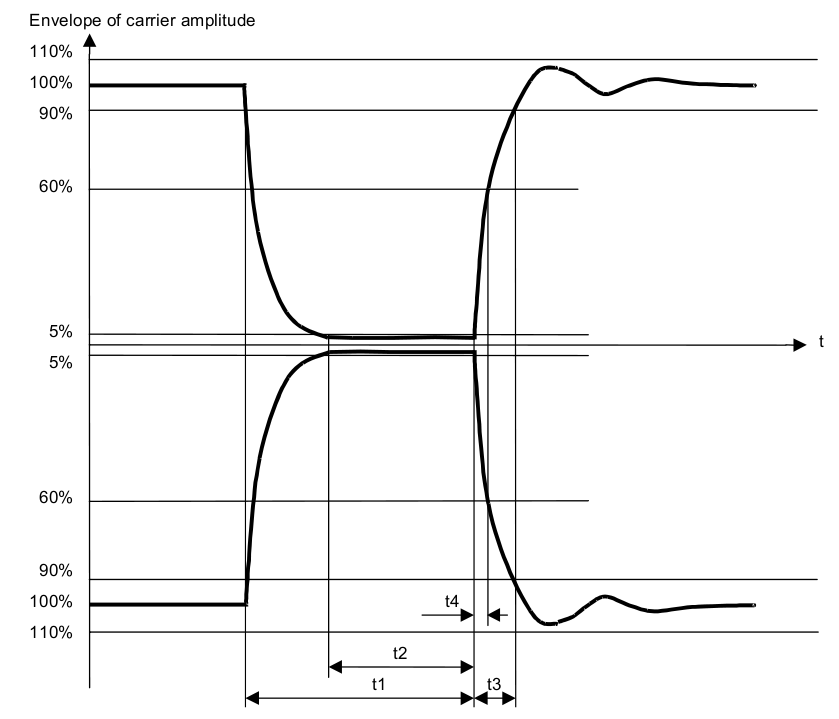
\includegraphics[scale=.4]{Imagenes/anexo1.png} 
  \end{center}
  \caption{Forma de pulso acorde a la norma ISO 14443}\label{Fig:pulso14443} 
\end{figure}


\subsection{Circuito receptor}

Cuando ya se han tomado en cuenta todos los cuidados en el diseño del transmisor, el circuito receptor debe ser conectado y ajustado.
Los valores de los componentes sugeridos en el circuito receptor son los siguientes:

\bigskip
	$C_{3} = 1nF$ 			(Ceramic NP0, tolerance $\leq \pm 10\%$) 
	
	$C_{4} = 100nF$ 			(Ceramic X7R, tolerance $\leq \pm 10\%$) 
	
	$R_{1} = 470 \Omega {...} 4.7 k \Omega $ 
	
	$R_{2} = 820 \Omega $
	
\bigskip
Dos reglas deben ser tenidas en cuenta para este circuito:

\begin{itemize}
\item[i.] El nivel de tensión de continua, DC, en la entrada Rx tiene que ser mantenido a $V_{mid}$ (por eso es necesario $R_{2}$ y $C_{4}$, ver figura \ref{Fig:RFID4}).
\item[ii.] El nivel de tensión de alterna, AC, en la entrada Rx debe ser mantenido entre los siguientes límites: $1,5V_{pp} < V_{Rx} < 3,0V_{pp}$.
\end{itemize}	

\bigskip
Si $V_{Rx} > 3,0V_{pp}$,  $R_{1}$ debe ser incrementada.

\bigskip
Si $V_{Rx} < 1,5V_{pp}$,  $R_{1}$ debe ser decrementada.

\bigskip
El voltaje a la entrada Rx debe ser verificado con y sin presencia de una tarjeta entre los límites máximo y mínimo de distancia de operación.

\bigskip
\begin{itshape}
El valor límite  $V_{Rx}= 3,0V_{pp}$ no debe ser excedido, un valor mayor puede causar fallos en la recepción.
\end{itshape}

\bigskip
\bigskip
\leftline{\bf{Otros puntos a tener en cuenta}}

\bigskip
\leftline{PCB}

\bigskip
La parte más crítica de todo el circuito analógico es el directamente conectado al integrado, o sea el filtro pasa bajos y la conexión de TVDD a la fuente de alimentación.
Entonces, por un lado un filtro puede ser usado para la conexión a la fuente de alimentación.
Por otro lado el diseño del filtro a la salida del integrado, formado por $L_{0}$ y $C_{0}$, debe ser considerado con mucho cuidado. \begin{itshape} El área y la distancia del filtro al integrado deben ser mantenidas lo más pequeñas posibles. Es recomendado además un plano de tierra.	
\end{itshape}

\bigskip
La figura \ref{Fig:RFID4} muestra un esquemático del diseño de una antena:

\begin{figure}[H]
\centering
  \begin{center}
  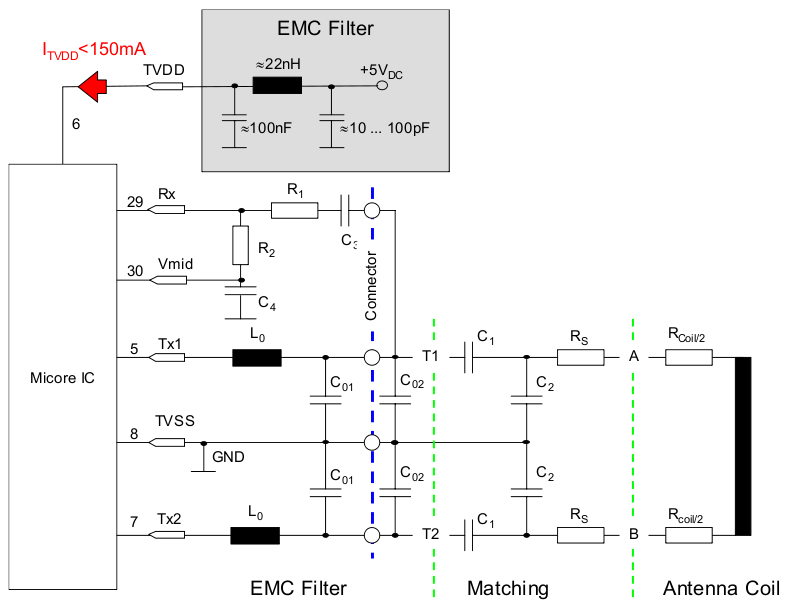
\includegraphics[scale=.4]{Imagenes/anexo2.png} 
  \end{center}
  \caption{Esquema de una antena, identificando sus principales secciones}\label{Fig:RFID4} 
\end{figure}


\bigskip
\leftline{Filtro de entrada de alimentación}

\bigskip
Aunque no sería necesario, un filtro puede ser conectado a la entrada TVDD para mejorar los siguientes puntos:

\begin{itemize}
\item[a)] suprimir ruido llegado desde la fuente de alimentación.
\item[b)] suprimir armónicos provenientes desde el transmisor.
\end{itemize}

Filtros idénticos pueden ser ubicados en las entradas AVDD y DVDD.

\newpage
\leftline{Blindaje}

\bigskip
El blindaje eléctrico absorbe el campo eléctrico generado por la antena. Para construir un blindaje, es recomendable usar un PCB de al menos 4 capas, donde el loop del blindaje se encuentra en las 2 capas externas. Este loop no debe ser cerrado y debe estar conectado en su punto central al sistema de tierra mediante una vía. Los extremos de la bobina deben ser ruteados próximos entre sí para evitar inductancias adicionales.  La figura \ref{Fig:blindaje} da una idea de como debe ser un blindaje: 


\begin{figure}[H]
\centering
  \begin{center}
  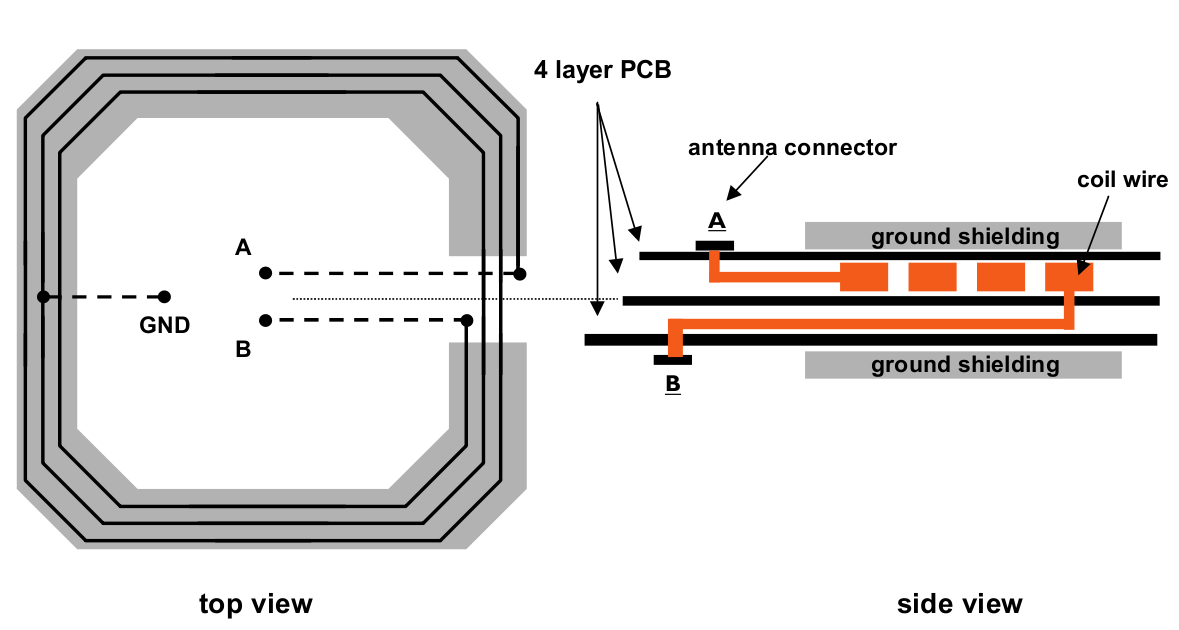
\includegraphics[scale=.3]{Imagenes/anexo3.png} 
  \end{center}
  \caption{Blindaje de una antena en un diseño de 4 capas}\label{Fig:blindaje} 
\end{figure}

